\subsection{Robustness and baseline comparison}
Across 12 synthetic conditions in which the actual Byzantine count and the generated honest coverage meet their specified allowances, the robust rule produced no observed wrong decisive classifications. Its mean decisive coverage was 87.52\%, compared with 75.63\% for the fixed-margin rule. These are observations under controlled assumptions, not estimates of failure rates in an actual vehicular deployment.

Table~\ref{tab:semantic} gives the focus condition, which uses calibrated correlated errors, maximum radius four, and one Byzantine issuer. The robust rule makes a decisive classification in 85.04\% of events, compared with 75.67\% for fixed margins. A median-point rule decides every event but produces 2.10\% false acceptance and 15.29\% false rejection. All-source intersection yields a high rate of evidence failure and can also make incorrect decisions, illustrating why requiring every source to agree is not inherently robust to adversarial observations.

\begin{table}[htbp]\centering\small
\caption{Focus-condition classification results: means over 30 seeds of 80 events each (percent). FA/FR use outside/inside denominators; the other columns use all events.}\label{tab:semantic}
\begin{tabular}{lrrrrr}\toprule
Method&FA&FR&Amb.&Failure&Decisive\\\midrule
Median point claim&2.10&15.29&0&0&100\\
Majority center&2.10&16.30&0&0&100\\
Fixed maximum-radius margin&0&0&24.33&0&75.67\\
All-source intersection&8.64&47.55&0&87.63&12.38\\
Robust feasible set&0&0&14.96&0&85.04\\\bottomrule
\end{tabular}\end{table}

A paired bootstrap with 10,000 resamples, using each random seed's paired outcomes as the resampling unit, estimates a 9.38-percentage-point increase in decisive coverage for the robust rule over fixed margins. The 95\% bootstrap percentile interval is 8.25--10.54 percentage points. This interval describes the difference for the specified synthetic workload; it is not a confidence statement about the population of real-world road conditions.

To check the theorem's premise explicitly, we group outcomes by the number $M$ of honest boxes that miss the true state. In the focus condition, all 2,400 events satisfy $M=0$, and no wrong decisive result was observed. Events sharing one random seed may be dependent, however, so 2,400 event records are not treated as independent trials proving a zero population error rate. Taking each seed's group of 80 events as one unit, and treating the presence of at least one wrong decisive result within that group as a Bernoulli failure, zero failures in 30 independent seed groups gives a one-sided 95\% exact binomial upper bound of 9.50\% on the group-level failure probability. That bound still applies only to the fixed synthetic generator.

Under the undercoverage error model, the fractions of events satisfying $M\le r$ are 52.42\%, 62.79\%, and 73.42\% for $r=0,1,2$, respectively. No wrong decisive classifications were observed among those satisfying the premise. Among events with $M>r$, the corresponding wrong-decisive rates were 1.31\%, 0.67\%, and 0.47\%. These diagnostics show that errors \emph{may} occur when the sufficient premise of Proposition~\ref{prop:soundness} is violated; they do not establish that every such violation causes an error, nor do they estimate the frequency of physical-premise failure in the field.

\begin{figure}[htbp]\centering
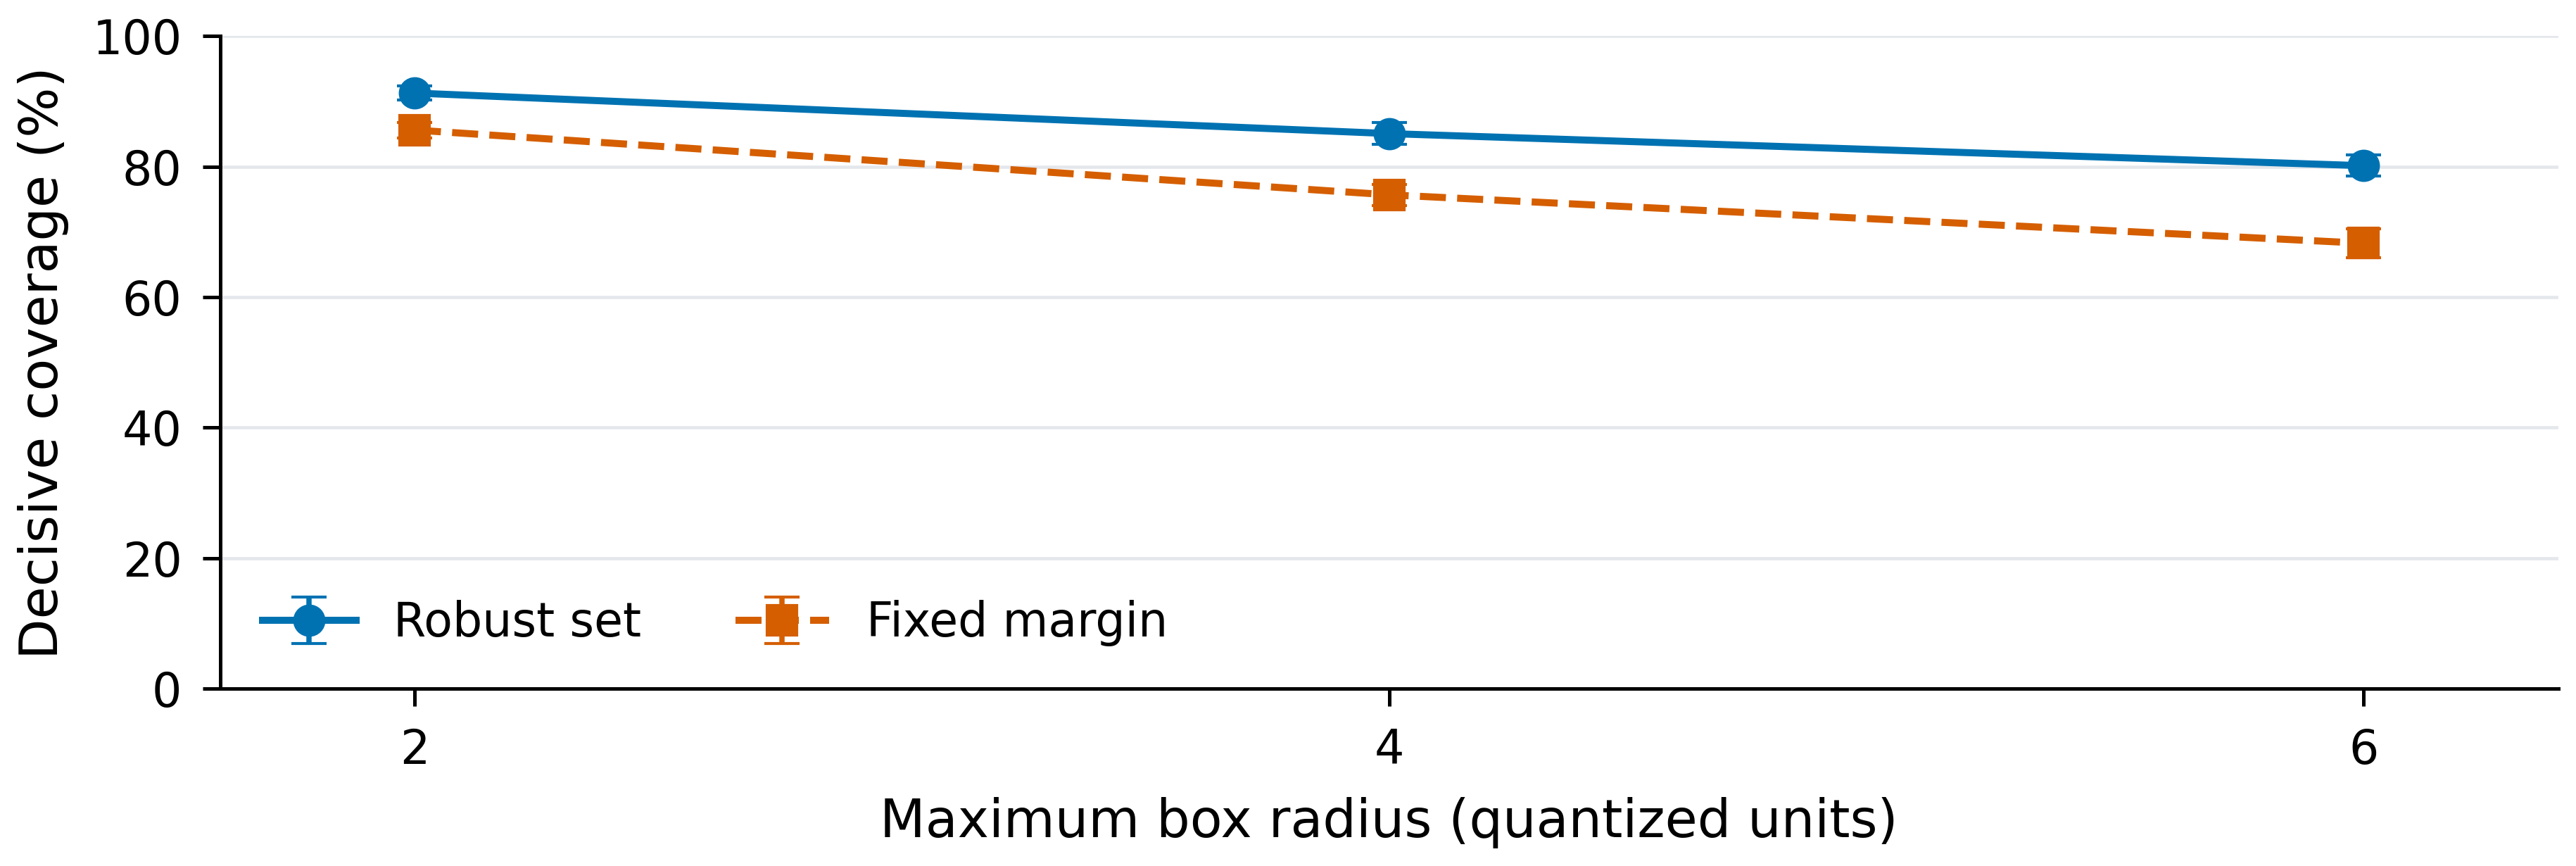
\includegraphics[width=\linewidth]{../figures/availability.png}
\caption{Decisive coverage versus maximum uncertainty radius for correlated calibrated errors with one Byzantine issuer. Error bars are normal-approximation 95\% intervals over 30 seed-level rates. Radius is expressed in quantized units, not calibrated physical distance.}\label{fig:availability}
\end{figure}

\subsection{Ablation and out-of-budget stress tests}
Table~\ref{tab:assumption-stress} examines two distinct violations of the stated assumptions. Honest-source undercoverage can produce wrong decisive results even when the number of Byzantine issuers remains within $f=1$. When two issuers are Byzantine but the verifier still assumes a budget of one, false acceptance, false rejection, and evidence failure all rise markedly. Inconsistent evidence therefore denotes an empty threshold-supported set, not a general detector of every fault-budget or calibration violation.

\begin{table}[htbp]\centering\small
\caption{Stress conditions violating source assumptions: means over 30 seeds (percent).}\label{tab:assumption-stress}
\begin{tabularx}{\linewidth}{@{}Xrrrr@{}}\toprule
Condition&FA&FR&Evidence failure&Decisive\\\midrule
Honest undercoverage; Byzantine count within budget&0.23&3.41&0&84.92\\
Two actual Byzantine issuers with verifier budget $f=1$&11.62&60.86&83.33&16.67\\\bottomrule
\end{tabularx}\end{table}

Table~\ref{tab:miscoverage} varies the allowed honest miscoverage $r$ while holding the observed evidence fixed. Under calibrated evidence, increasing $r$ from zero to two lowers decisive coverage from 85.04\% to 77.46\%, without observed wrong decisive decisions. For undercovered evidence, a larger $r$ accompanies a reduction in false rejection from 3.41\% to 0.94\%, while decisive coverage falls from 84.92\% to 78.50\%. With $n$ and $f$ fixed, increasing $r$ reduces $k=n-f-r$ and expands $\mathcal F_k$. It is then harder for \emph{every} feasible state to lie within the authorized policy. Thus changing the allowance alters decision conservatism but does not improve physical sensor calibration.

\begin{table}[htbp]\centering\small
\caption{Paired ablation over honest-miscoverage allowance ($n=5$, $f=1$, maximum radius four, one Byzantine issuer; percent).}\label{tab:miscoverage}
\begin{tabular}{lrrrr}\toprule
Error model&$r$&FA&FR&Decisive coverage\\\midrule
Calibrated&0&0&0&85.04\\
Calibrated&1&0&0&81.25\\
Calibrated&2&0&0&77.46\\
Undercovered&0&0.23&3.41&84.92\\
Undercovered&1&0&1.79&81.67\\
Undercovered&2&0&0.94&78.50\\\bottomrule
\end{tabular}\end{table}

\begin{figure}[htbp]\centering
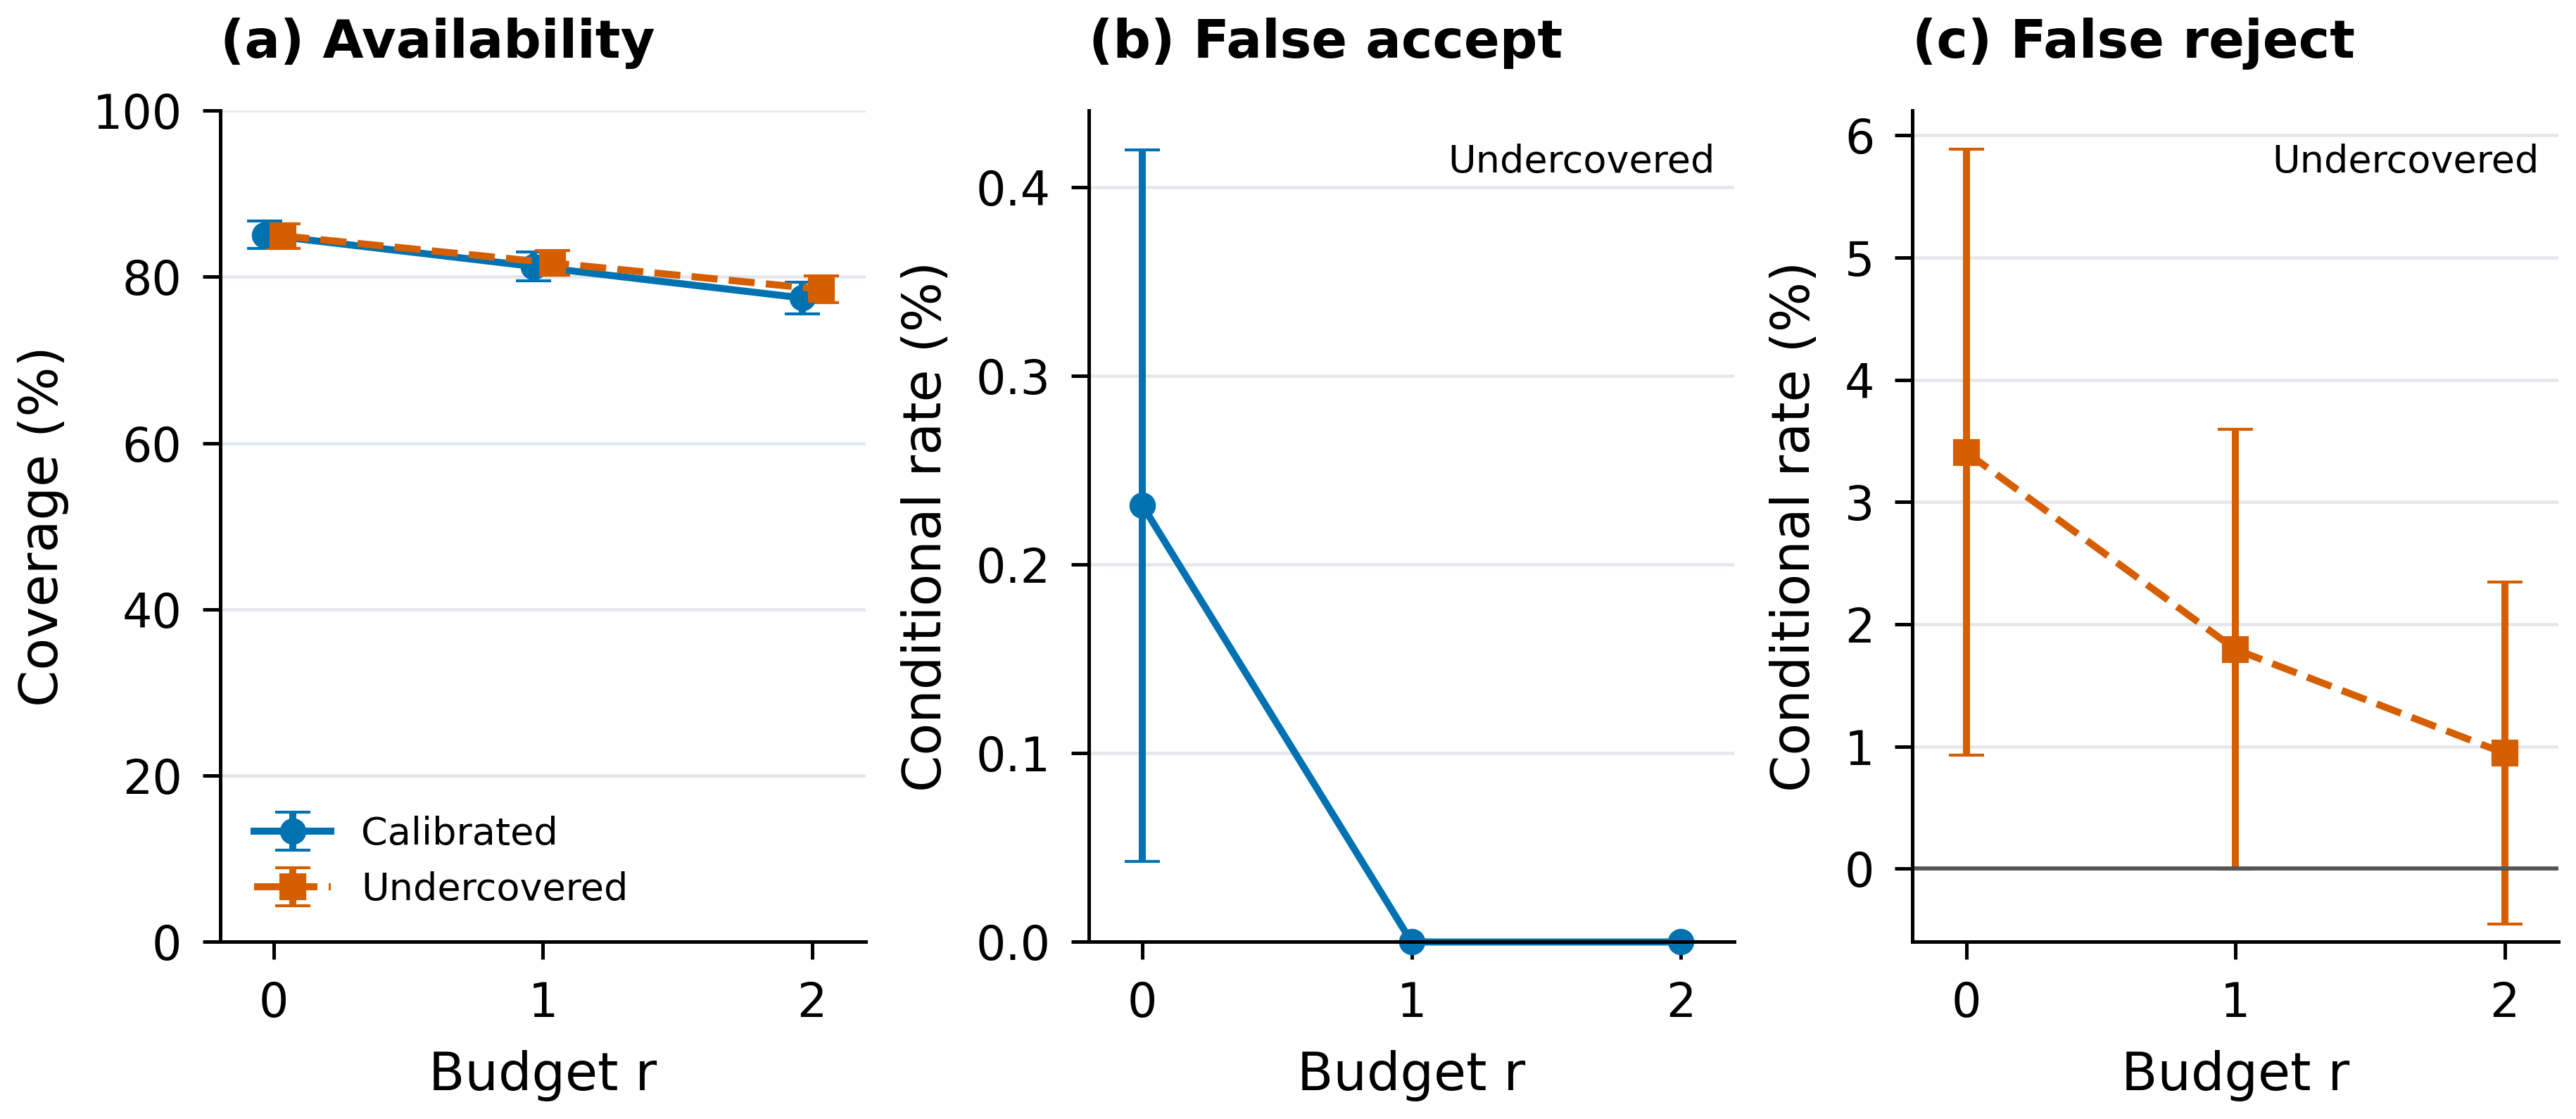
\includegraphics[width=\linewidth]{../figures/budget_tradeoff.png}
\caption{Effects of the honest-miscoverage allowance $r$ for $n=5$, $f=1$. Points are means over the same 30 seeds; error bars are normal-approximation 95\% intervals. Zero-width intervals for observed zero errors do not imply a population error probability of zero; occasional negative plotted interval endpoints arise from the normal approximation.}\label{fig:budget}
\end{figure}

Replay over a measured reference path provides a complementary test. With nominal simulated evidence along UrbanNav, the robust rule achieves 93.27\% decisive coverage, compared with 81.94\% for fixed margins; neither produced observed errors. The median-point rule has 0.29\% false acceptance and 3.12\% false rejection. When the simulated common-mode bias is multiplied by four, the robust rule exhibits 0.032\% false acceptance and 0.493\% false rejection. All of these figures describe simulated evidence on a measured trajectory, not calibration of real multisensor hardware. In particular, the 77.46\% value in Table~\ref{tab:miscoverage} belongs to the synthetic $r=2$ ablation, not to UrbanNav under common-mode bias.
